% ------------------------------------------------------------------------------
% Palestra: Como os tradutores inativos do GNOME foram separados dos ativos
% Autores:
%     Adorilson Bezerra <adorilson@gmail.com>
% Licen�a Creative Commons Atribui��o 3.0. 
% Voc� pode usar e alterar este documento, 
% mas deve obrigatoriamente citar a autoria. 
% ------------------------------------------------------------------------------

\documentclass{beamer}

% ------------------------------------------------------------------------------
\usepackage[latin1]{inputenc}
\usepackage[brazil]{babel}
\usepackage{graphicx}
\usepackage{beamerthemesplit}
\usepackage{ae}
\usepackage{alltt}
\usepackage{pslatex}
% ------------------------------------------------------------------------------

\usecolortheme{beaver}

% ------------------------------------------------------------------------------
\title[Introdu��o ao desenvolvimento de software livre]
{
    Introdu��o ao desenvolvimento de software livre
}
\subtitle{Li��es aprendidas com hacking no Damned Lies}
\author[Adorilson Bezerra]
{
    Adorilson Bezerra
}
\date{\today}
\logo{
\includegraphics{img/gnome-gtp}}
% ------------------------------------------------------------------------------

\begin{document}

% ------------------------------------------------------------------------------
\frame{\titlepage}
% ------------------------------------------------------------------------------
\frame
{
    \frametitle{Ado... o que?}
    
    \begin{columns}
        \column{0.4\textwidth}
        \begin{itemize}
            \item adorilson @ internet
            \item adorilson.bezerra no ifrn.edu.br
        \end{itemize}
        \column{0.4\textwidth}
        
\includegraphics[scale=0.3]{img/hackergotchi}
    \end{columns}
}

% ------------------------------------------------------------------------------
\section{Introdu��o}

\subsection{Sobre o software livre}
\frame
{
    \frametitle{O software � livre se voc� tem a liberdade para...}
    \begin{itemize}
        \item ... executar o programa para qualquer prop�sito
        \item ... estudar como o programa funciona e adapt�-los para suas necessidades
        \item ... redistribuir c�pias de modo que voc� possa ajudar ao seu pr�ximos
        \item ... aperfei�oar o programa, e liberar os seus aperfei�oamentos, de 
        modo que toda a comunidade se beneficie
    \end{itemize}
}


\frame
{
    \frametitle{Motiva��o}
    \begin{columns}
        \column{0.4\textwidth}
        \begin{itemize}
            \item "Pagamento", retribui��o
            \item Necessidade
            \item Aprendizado
            \item Divers�o, realiza��o
            \item ...
        \end{itemize}
        \column{0.4\textwidth}
        \begin{figure}[t]
            \centering
            
\includegraphics[scale=0.4]{img/challenge-accepted}
        \end{figure}
    \end{columns}
}

\frame
{
    \frametitle{Estudo de caso}
    \begin{quote}
        Como os tradutores inativos do GNOME foram separados dos ativos
    \end{quote}
}

\subsection{Sobre o GNOME}
\frame
{
    \frametitle{O GNOME �...}
        
    
    \begin{columns}
        \column{0.7\textwidth}
        \begin{quote}
        ... um projeto Internacional de software livre que prov� basicamente duas solu��es: o ambiente desktop GNOME, intuitivo e atraente para usu�rios finais; e a Plataforma de Desenvolvimento GNOME, um framework extenso para constru��o de aplica��es que se integrem com todo o desktop. (Fonte: http://br.gnome.org/)
        \end{quote}
        \column{0.4\textwidth}
        \begin{figure}
            \centering
            
\includegraphics[scale=0.5]{img/gnome}
        \end{figure}
    \end{columns}
}

\subsection{Sobre o damned-lies}
\frame
{
    \frametitle{http://l10n.gnome.org}
    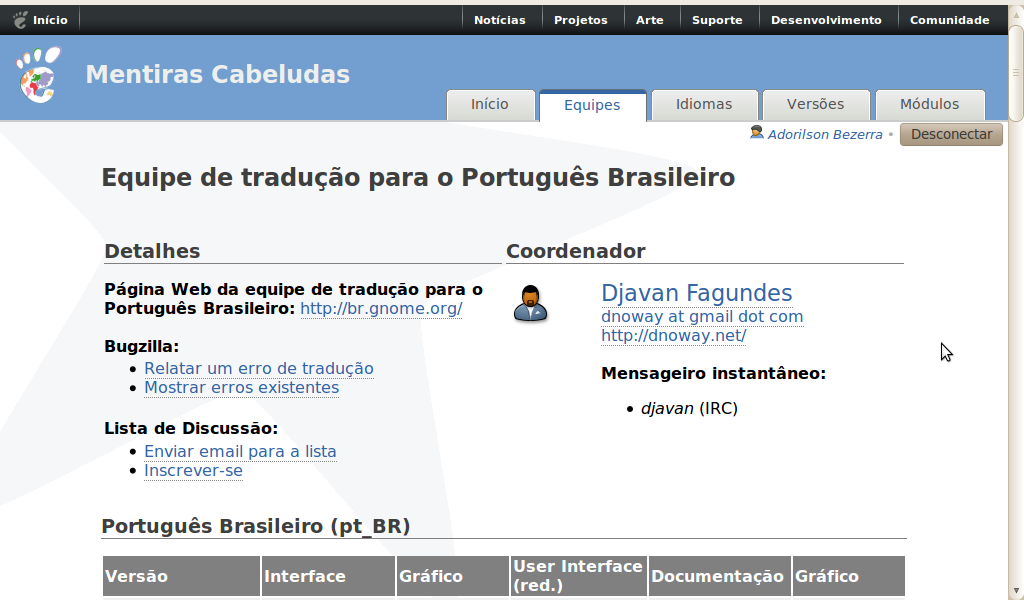
\includegraphics[scale=0.3]{img/dl}
}

\subsection{O Problema}
\frame
{
    \frametitle{Separar tradutores ativos e inativos}
    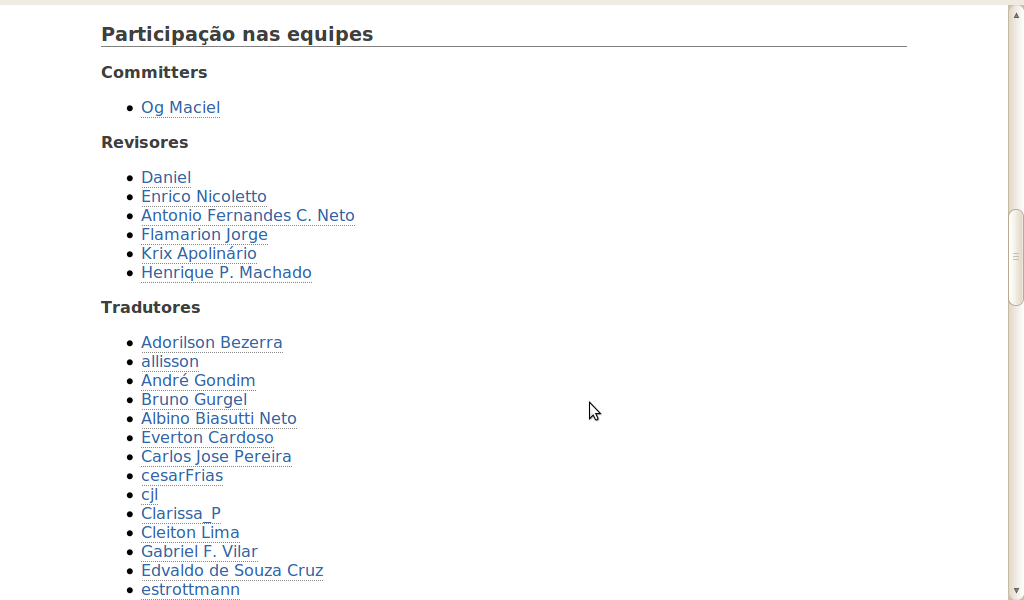
\includegraphics[scale=0.3]{img/dl2}
}

% ------------------------------------------------------------------------------
\subsection{O start}
\frame
{
    \frametitle{Eventos rocks!!!}
    \begin{columns}
        \column{0.4\textwidth}
        \begin{figure}[t]
            \centering
            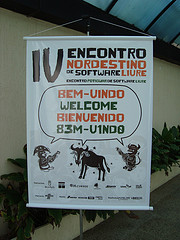
\includegraphics[width=4.5cm]{img/ensl}
        \end{figure}
        \column{0.4\textwidth}
        \begin{figure}[t]
            \centering
            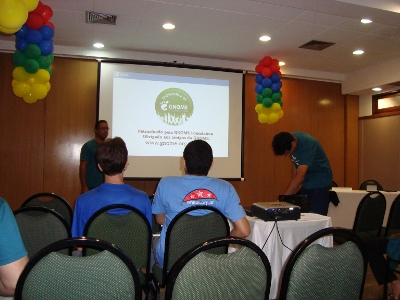
\includegraphics[width=4.5cm]{img/gnome2}
        \end{figure}
        \column{0.4\textwidth}
        \begin{figure}[t]
            \centering
            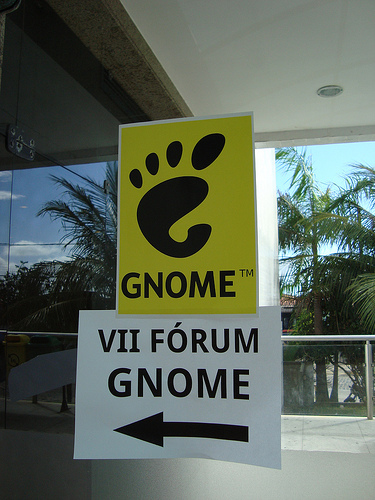
\includegraphics[width=4.5cm]{img/gnome1}
        \end{figure}
    \end{columns}
    {\tiny Fotos por: Krix Apolin�rio (\url{http://blog.krix.com.br/2010/11/iv-ensl-e-vii-forum-gnome-\%e2\%80\%93-parte-22/})}
}
\frame
{
    \frametitle{Cria��o do bug em http://bugzilla.gnome.org => http://vai.la/2aqc}
    \begin{figure}[t]
        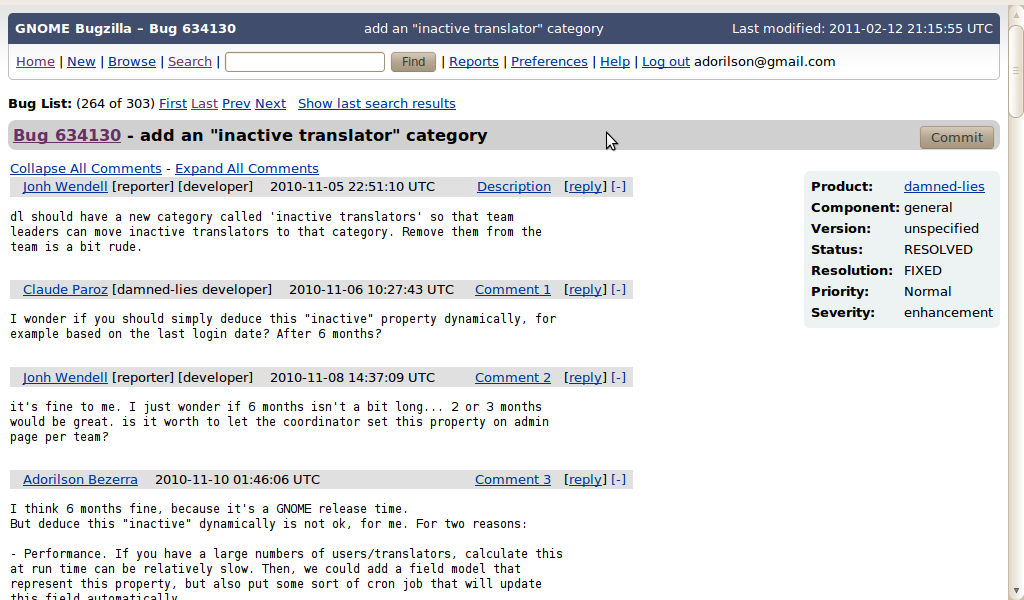
\includegraphics[scale=0.5]{img/bugzilla}
    \end{figure}
}

% ------------------------------------------------------------------------------

\section{Desenvolvimento}
\frame
{
    \frametitle{Du iu ispique inglishe?}
    \begin{figure}[t]
        
\includegraphics{img/flag_usa}
    \end{figure}
}
\frame
{
    \frametitle{Ferramentas}
    \begin{figure}[t]
        
\includegraphics[scale=0.6]{img/python_django}
    \end{figure}
}
\frame
{
    \frametitle{IRC vive}
    \begin{figure}[t]
        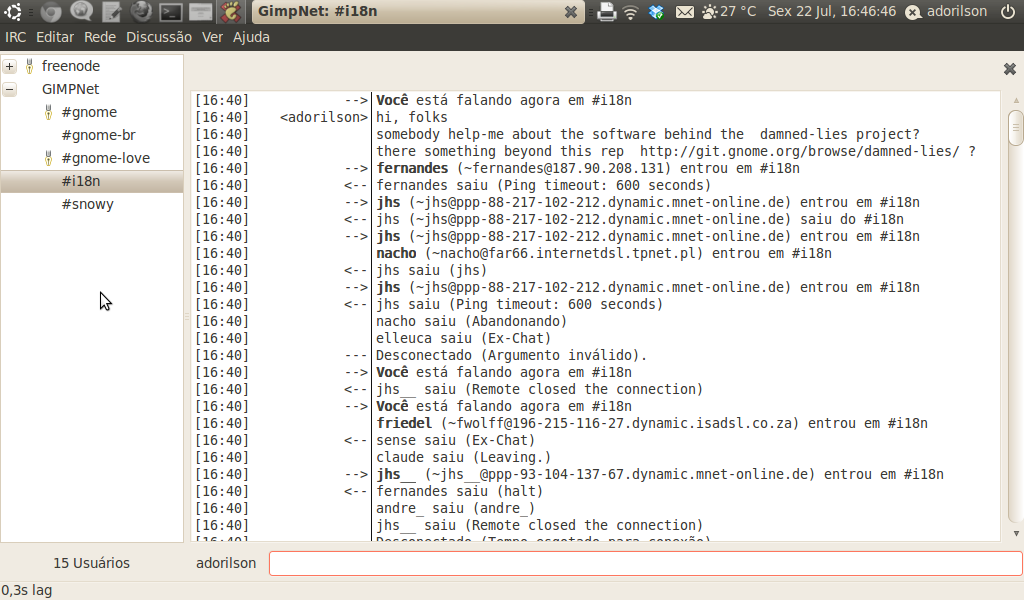
\includegraphics[scale=0.3]{img/irc}
    \end{figure}
}
\frame
{
    \frametitle{Discuta}
    \begin{figure}[t]
        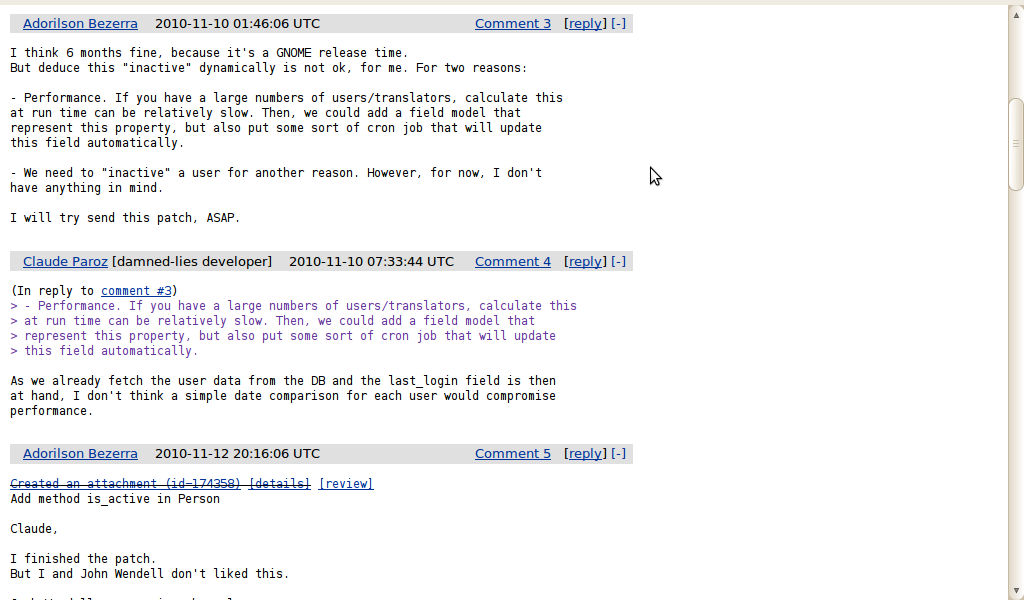
\includegraphics[scale=0.4]{img/discuta}
    \end{figure}    
}
\frame
{
    \frametitle{Show me the code}
    \begin{figure}[t]
        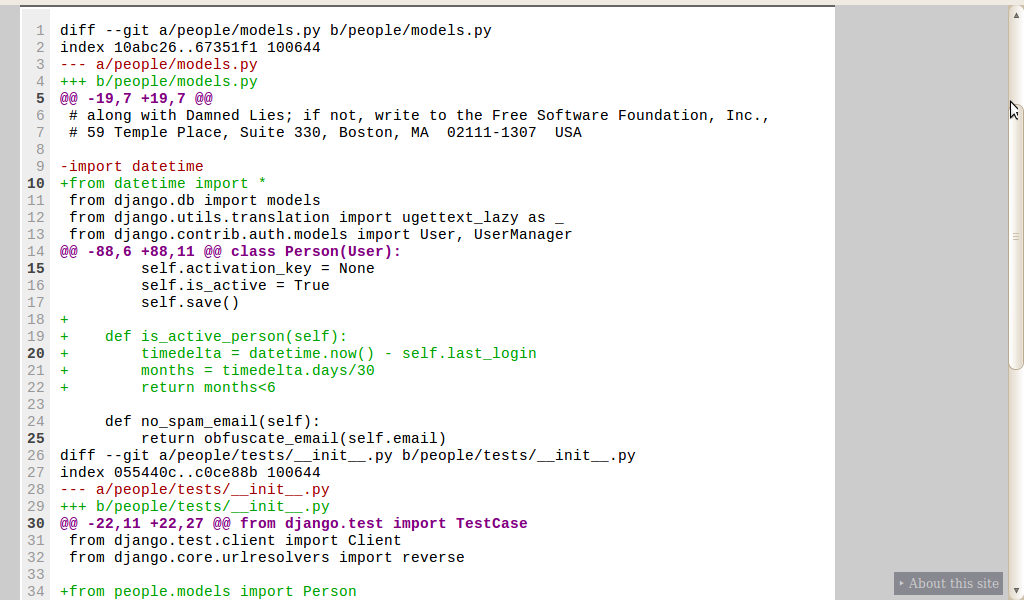
\includegraphics[scale=0.4]{img/patch1}
    \end{figure}
}
\frame
{
    \frametitle{Consiga um apoio}
    \begin{figure}[t]
        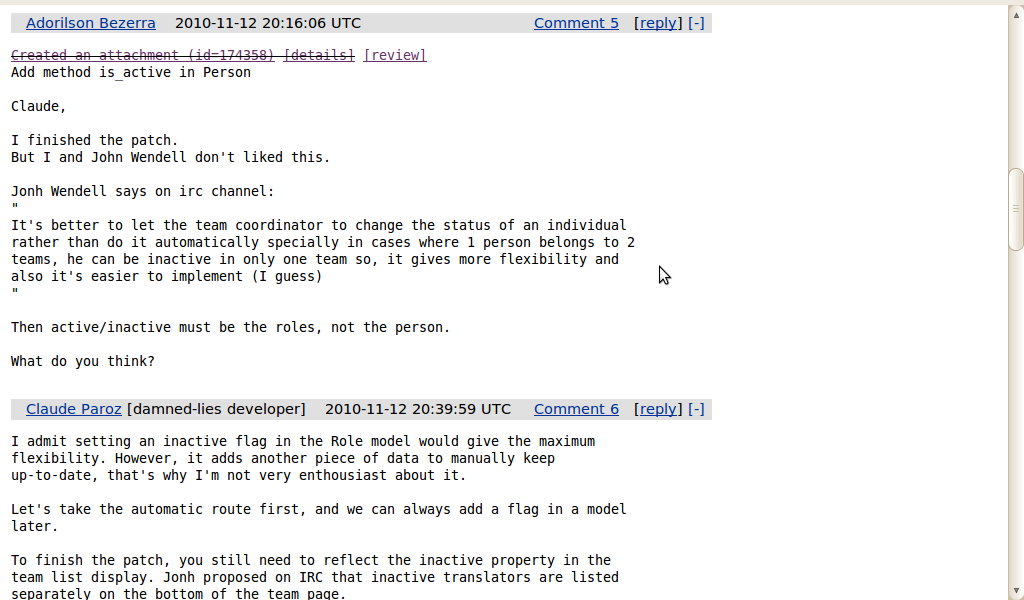
\includegraphics[scale=0.4]{img/mentor}
    \end{figure}
}
\frame
{
    \frametitle{Aprenda}
    \begin{figure}[t]
        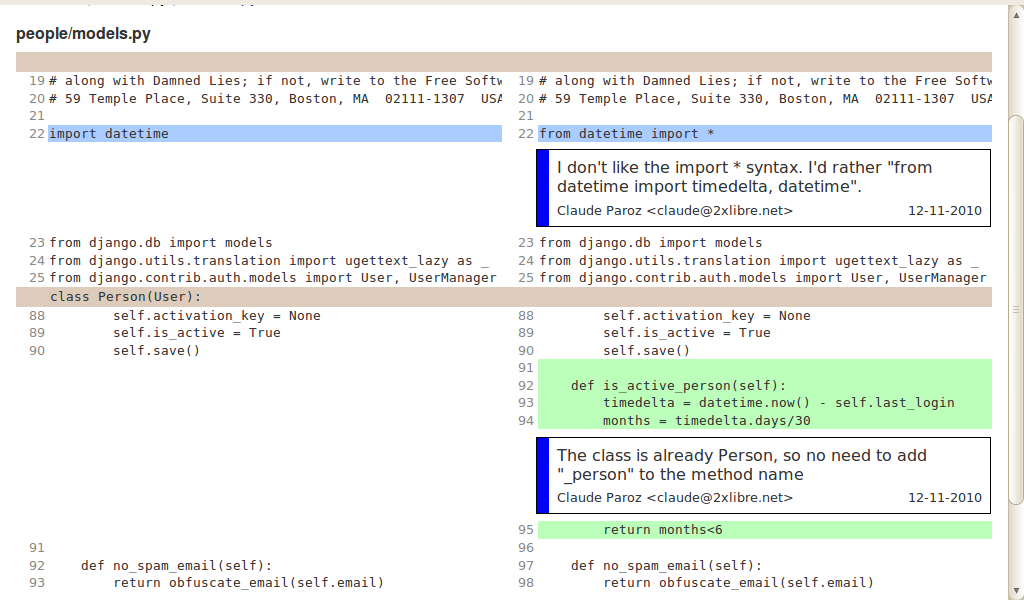
\includegraphics[scale=0.3]{img/aprenda}
    \end{figure}
}
\frame
{
    \frametitle{Cultive o desapego ao c�digo}
    \begin{figure}[t]
        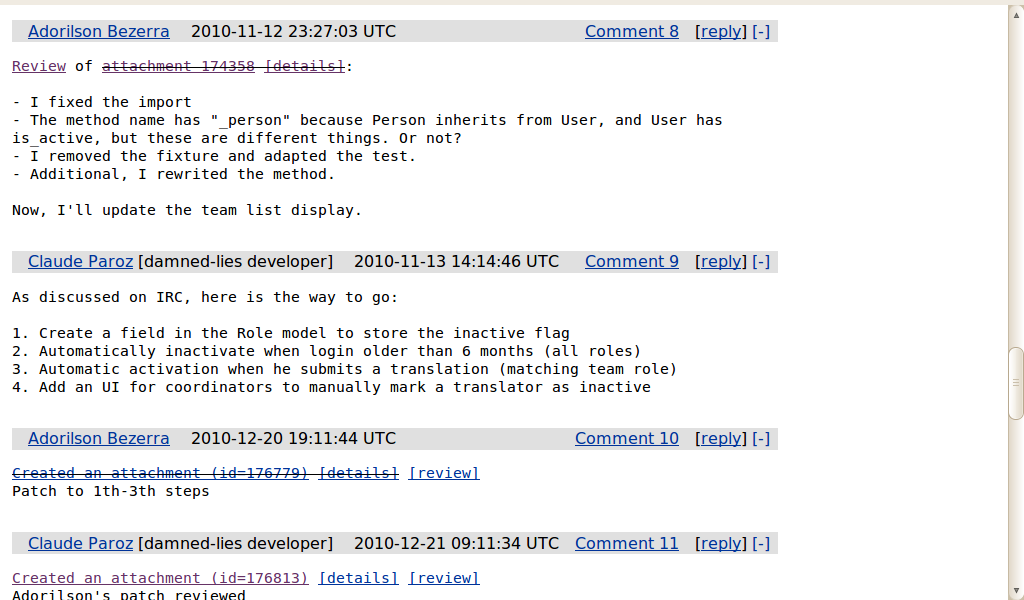
\includegraphics[scale=0.4]{img/desapego}
    \end{figure}
}
\frame
{
    \frametitle{Envolva-se mais}
    \begin{figure}[t]
        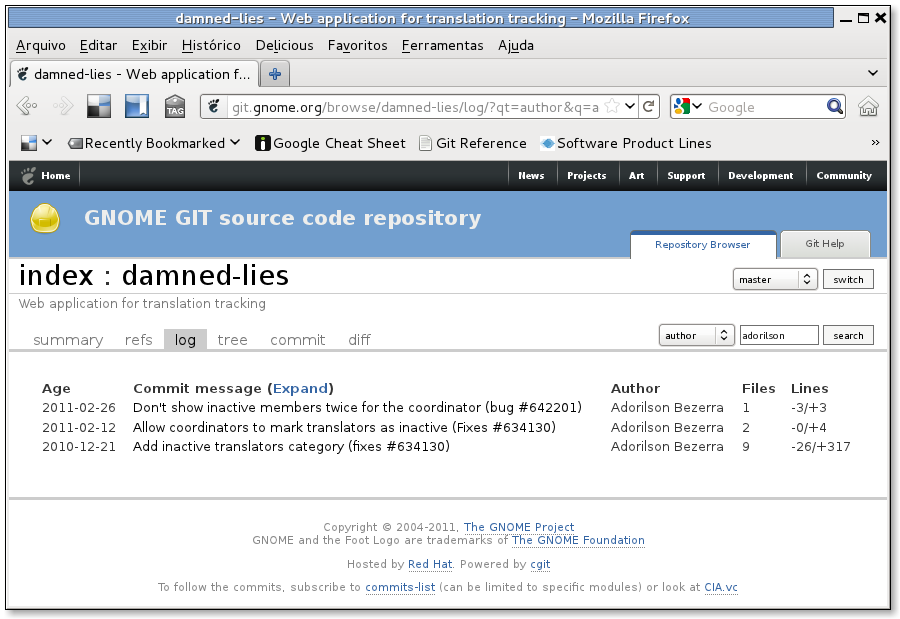
\includegraphics[scale=0.3]{img/outras_contribuicoes}
    \end{figure}
}
\frame
{
    \frametitle{Participe da governan�a}
    \begin{figure}[t]
        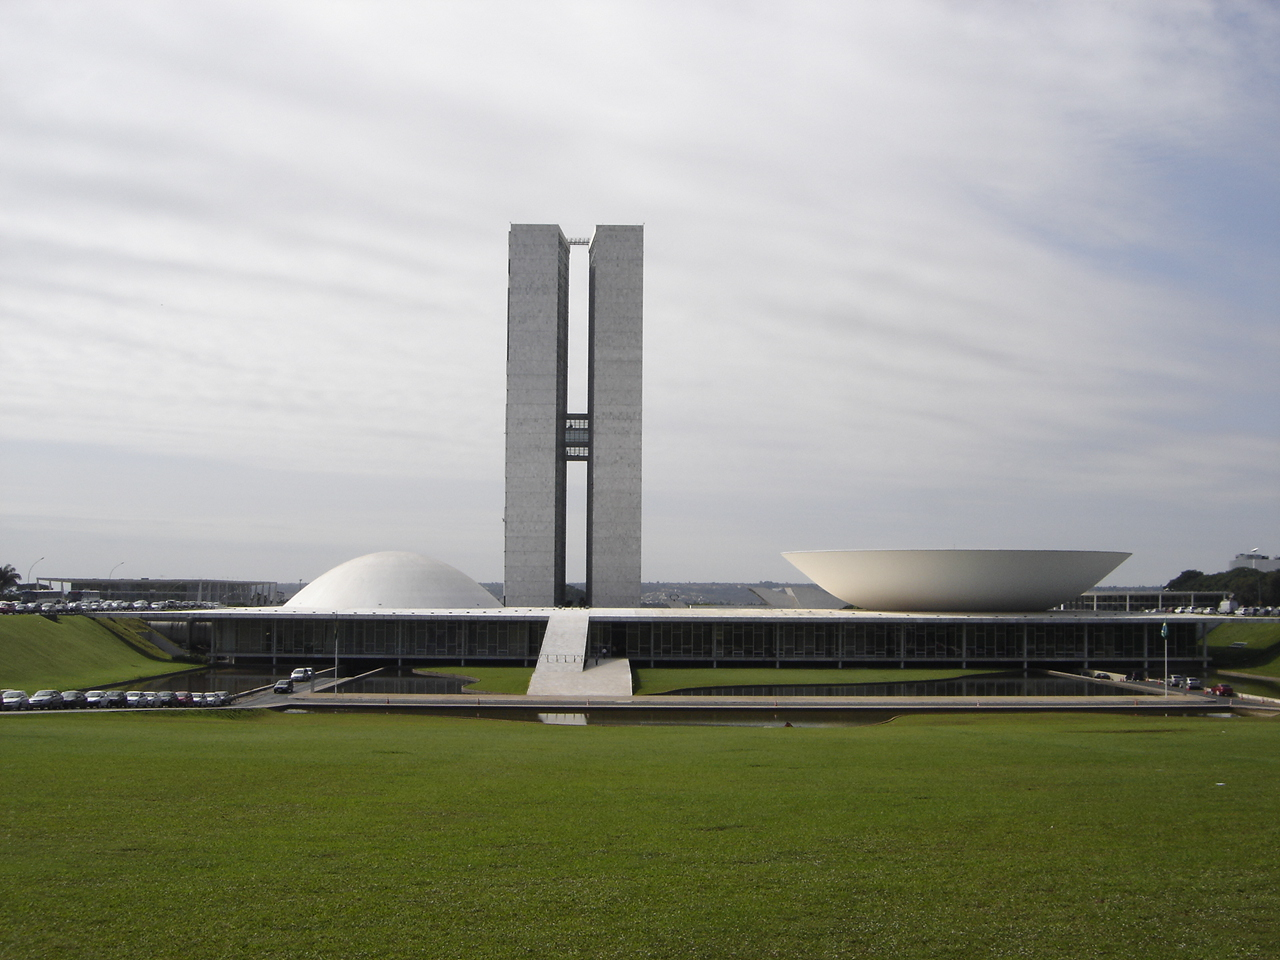
\includegraphics[scale=0.25]{img/brasilia}
    \end{figure}
}
\frame
{
    \frametitle{Espalhe}
    \begin{figure}[t]
        
\includegraphics[scale=0.5]{img/espalhe}
    \end{figure}
}

\section{Conclus�o}
\frame
{
    \frametitle{Software livre � bom para voc�}
    \begin{figure}[t]
        
\includegraphics[scale=0.6]{img/softwarelivre}
    \end{figure}
}

\frame{
	\frametitle{GNOME Goals (Slide b�nus)}
	\begin{figure}[t]
		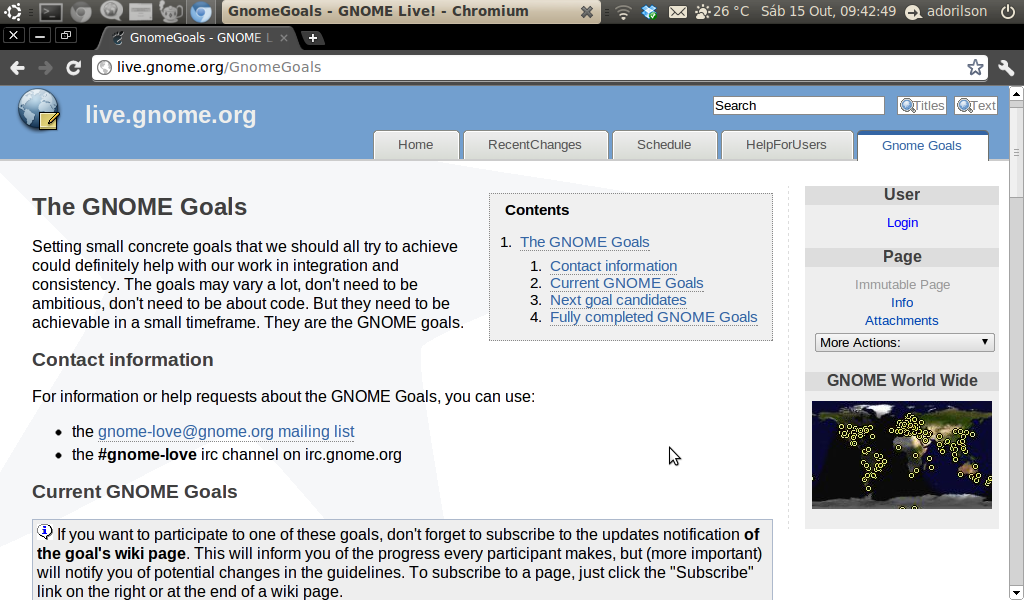
\includegraphics[scale=0.3]{img/gnome_goals}
	\end{figure}
}

\frame{
	\frametitle{Indica��o de leitura para o fim de semana}
	\begin{itemize}
	    \item Colabora��o e Open Source dentro da empresa - Guilherme Chapiewski
	            \begin{itemize}
                    \item http://vai.la/2uIi
                \end{itemize}
        \item Catedral e o Bazar - Eric Raymond
                \begin{itemize}
                    \item http://vai.la/2uHM
                 \end{itemize}
	\end{itemize}
}

\end{document}
